\chapter{Conception et architecture}
\label{chap:conception}

\section*{Introduction}

Ce chapitre présente l'architecture retenue et justifie les choix technologiques. L'accent est
mis sur les décisions structurantes --- celles qui, une fois prises, contraignent tout le reste
--- et sur les arbitrages assumés, y compris ceux qui restent discutables.

\section{Architecture générale}

Le système se décompose en deux pipelines distincts : un pipeline d'\textbf{indexation} exécuté
une seule fois hors ligne, et un pipeline de \textbf{requête} exécuté à chaque question.

\begin{figure}[H]
    \centering
    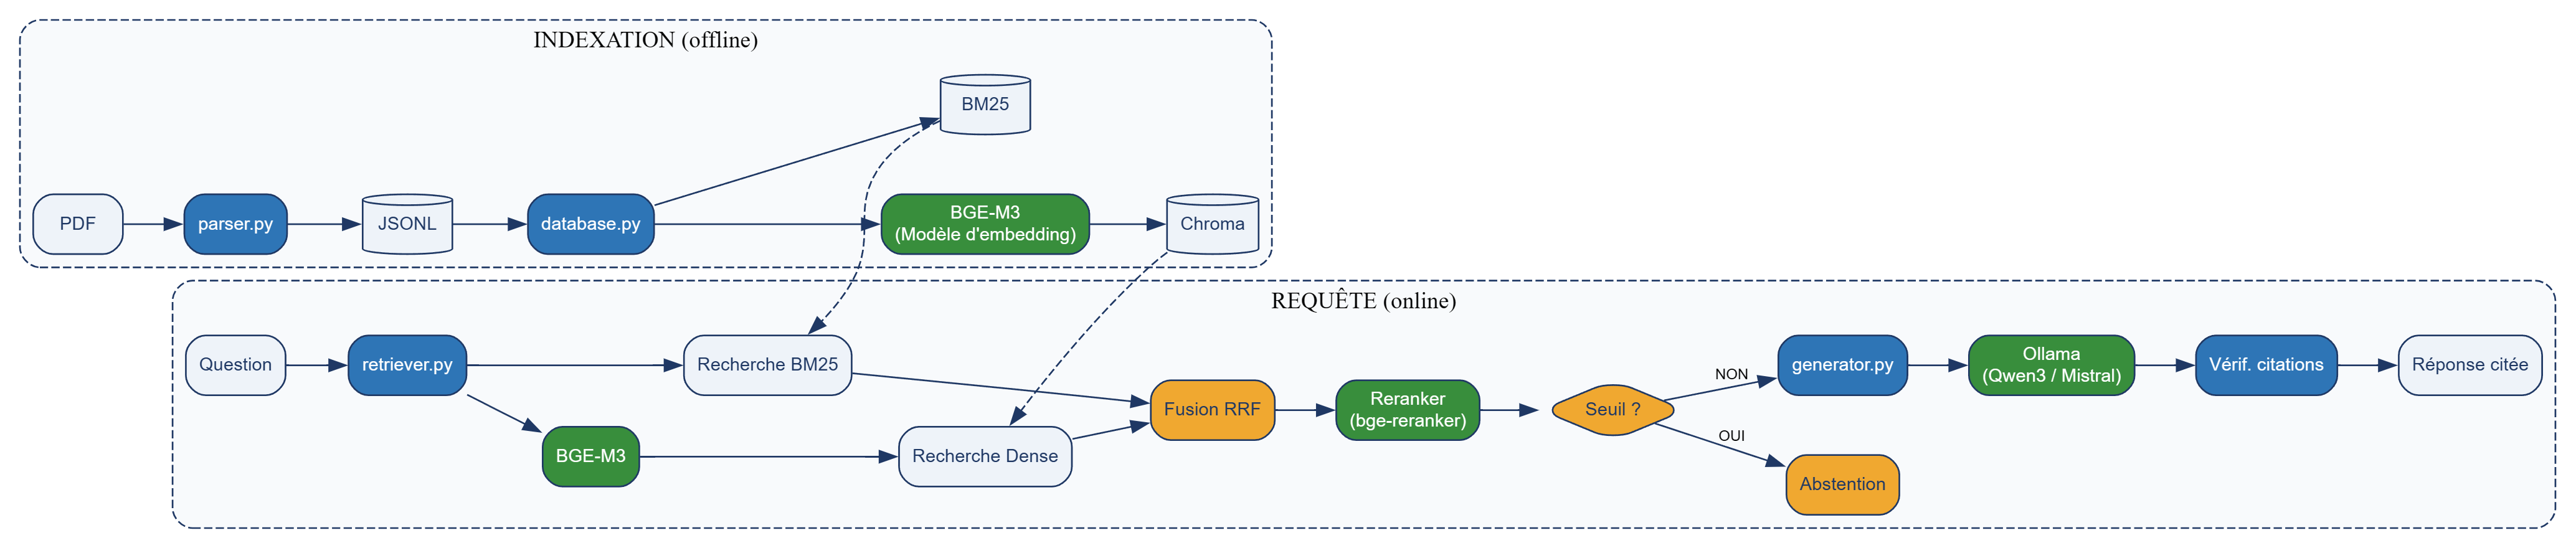
\includegraphics[width=\textwidth]{Figures/architecture.png}
    \caption{Architecture générale : pipeline d'indexation (hors ligne) et pipeline de requête (en ligne)}
    \label{fig:architecture}
\end{figure}

Les index Chroma (dense) et BM25 (lexical), construits hors ligne, sont ceux qu'interrogent
respectivement les recherches dense et lexicale du pipeline de requête. Le modèle d'embedding
BGE-M3 intervient \textbf{deux fois} : à l'indexation, pour vectoriser les articles ; à la
requête, pour vectoriser la question. C'est cette identité qui garantit que les deux vivent dans
le même espace vectoriel et que la comparaison a un sens.

\subsection{Deux principes structurants}

\paragraph{Le garde-fou d'abstention est placé \emph{avant} le modèle.}
Il s'agit d'un test de seuil sur le score de recherche, donc d'un mécanisme
\textbf{indépendant du modèle}. Il ne dépend pas de la bonne volonté du LLM à dire « je ne sais
pas » --- ce sur quoi les petits modèles locaux sont peu fiables. Ce choix a un effet secondaire
mesurable : lorsqu'il se déclenche, le modèle n'est pas appelé du tout, et la réponse est rendue
en une fraction du temps habituel (cf. chapitre~\ref{chap:evaluation}).

\paragraph{La recherche et la génération sont séparables.}
À tout moment il est possible d'afficher les articles retrouvés \emph{avant} l'appel au modèle.
Cette séparation rend le débogage possible : face à une mauvaise réponse, elle permet de
déterminer immédiatement si le problème vient de la recherche ou de la génération.

\section{Séquence d'une requête}

\begin{enumerate}
    \item L'orchestrateur reçoit la question de l'utilisateur.
    \item Il appelle la fonction de recherche.
    \item La question est vectorisée avec BGE-M3, puis les index Chroma et BM25 sont interrogés
    \textbf{en parallèle} ; les deux classements sont fusionnés par RRF.
    \item Le \textbf{garde-fou} est appliqué : si le meilleur score est sous le seuil calibré,
    l'abstention est immédiate et le modèle n'est pas appelé.
    \item Sinon, les articles retenus sont transmis au générateur.
    \item Le générateur construit un prompt strict, appelle le modèle local à basse température,
    puis \textbf{vérifie que chaque numéro d'article cité figure bien dans le contexte fourni}.
    \item L'orchestrateur affiche la réponse, les articles cités et l'avertissement d'usage.
\end{enumerate}

\section{Rôle de chaque module}

\begin{table}[H]
    \centering
    \begin{tabular}{|m{2.4cm}|m{5.2cm}|m{6.4cm}|}
        \hline
        \textbf{Module} & \textbf{Rôle} & \textbf{Entrée $\rightarrow$ Sortie} \\
        \hline
        \texttt{parser.py} & Extraction PDF, découpage par article, métadonnées & PDF source $\rightarrow$ corpus JSONL \\
        \hline
        \texttt{database.py} & Calcul des embeddings, construction de l'index & JSONL $\rightarrow$ collection Chroma \\
        \hline
        \texttt{retriever.py} & Recherche dense et lexicale, fusion RRF & Question $\rightarrow$ articles + scores \\
        \hline
        \texttt{generator.py} & Prompt ancré, appel au modèle local & Question + articles $\rightarrow$ réponse \\
        \hline
        \texttt{app.py} & Orchestration, abstention, vérification des citations & Question $\rightarrow$ réponse affichée \\
        \hline
    \end{tabular}
    \caption{Répartition des responsabilités entre modules}
    \label{tab:modules}
\end{table}

\subsection{Découplage et interchangeabilité}

Chaque composant est isolé derrière une fonction simple, ce qui permet de remplacer une brique
sans toucher aux autres :

\begin{itemize}
    \item Changer de modèle d'embeddings impose de modifier \texttt{database.py} \textbf{et}
    \texttt{retriever.py} --- les deux doivent impérativement utiliser le même modèle, faute de
    quoi question et articles ne vivent plus dans le même espace vectoriel.
    \item Changer de modèle de langage n'affecte que \texttt{generator.py}.
    \item Passer du dense seul à l'hybride n'affecte que \texttt{retriever.py}.
\end{itemize}

Cette contrainte est délibérée : elle rend l'\textbf{évaluation comparative} possible, en
permettant de ne mesurer qu'une variante à la fois.

\section{Choix technologiques}

\subsection{Deux filtres derrière chaque décision}

La quasi-totalité des choix découle de deux contraintes :

\begin{enumerate}
    \item \textbf{Souveraineté $\rightarrow$ tout doit s'exécuter en local.} Ce seul critère
    élimine les embeddings par API, les services de reclassement commerciaux et les modèles de
    génération propriétaires. Beaucoup de « pourquoi pas X ? » se résument à : \emph{X est une
    API ; la question du citoyen ne doit pas quitter le territoire}.
    \item \textbf{Corpus borné et durée courte $\rightarrow$ optimiser la compréhension et la
    maîtrise, pas la performance à grande échelle.} À l'échelle de quelques centaines d'articles,
    toutes les bases vectorielles sont instantanées : la performance brute n'est jamais le
    facteur décisif.
\end{enumerate}

\subsection{Décisions par composant}

\begin{longtable}[c]{| m{2.6cm} | m{3.1cm} | m{8.4cm} |}
\caption{Choix technologiques et justifications}\label{tab:techno}\\
\hline
\textbf{Couche} & \textbf{Choix} & \textbf{Justification} \\
\hline
\endfirsthead
\hline
\textbf{Couche} & \textbf{Choix} & \textbf{Justification} \\
\hline
\endhead
Extraction PDF & PyMuPDF & Rapide, fidélité Unicode fiable. Surtout : contrôle brut sur la façon dont la loi est découpée, là où les parseurs automatiques masquent ce contrôle. \\
\hline
Embeddings & BGE-M3 & La souveraineté exclut les embeddings par API. Parmi les modèles locaux : bonne couverture FR + AR, contexte long (8192 tokens, aucun article tronqué). \\
\hline
Base vectorielle & Chroma & À cette échelle la performance est hors sujet : l'expérience de développement a été privilégiée. Chroma est embarquée (pas de serveur), persiste sur disque, filtre par métadonnées. \\
\hline
Recherche lexicale & BM25 (\texttt{rank\_bm25}) & Les requêtes juridiques sont riches en tokens exacts (numéros d'articles, « Loi 65-99 ») --- précisément là où le lexical bat les embeddings. \\
\hline
Runtime LLM & Ollama & Une commande télécharge et sert un modèle quantifié via une API propre. \\
\hline
Modèle & Mistral 7B & La souveraineté exclut les modèles frontières par API. La classe 7B est le point d'équilibre : suffisante en suivi d'instructions, exécutable sur du matériel étudiant. Mistral pour la qualité du français. \\
\hline
Framework RAG & \textbf{Aucun} & Pour un corpus borné, la boucle RAG représente environ 150 lignes. La coder soi-même permet de comprendre chaque étape, de déboguer directement, et d'expliquer son propre pipeline en soutenance. \\
\hline
Format du corpus & JSONL & Un article par ligne : lisible, métadonnées imbriquées, \emph{diff-able} sous Git, lecture en flux. \\
\hline
\end{longtable}

\subsection{Les arbitrages réellement discutables}

Il serait malhonnête de présenter tous ces choix comme évidents. Trois d'entre eux restent
ouverts :

\begin{itemize}
    \item \textbf{BGE-M3 contre multilingual-e5} --- appel serré ; e5 est plus léger. BGE-M3
    l'emporte sur la largeur multilingue et la longueur de contexte.
    \item \textbf{Sans framework contre LlamaIndex} --- l'arbitrage le plus discutable. Un
    framework se justifierait si le projet grossissait (sources multiples, agents, routage).
    \item \textbf{Dense seul contre hybride} --- l'hybride est peu coûteux et le texte juridique
    favorise la correspondance exacte ; mais la position honnête est \emph{« je l'ai mesuré,
    voici l'écart »}. Le chapitre~\ref{chap:evaluation} montre que cet écart n'est pas celui
    attendu.
\end{itemize}

\newpage
\section*{Conclusion}

L'architecture retenue place délibérément le garde-fou d'abstention hors du modèle et maintient
la recherche séparable de la génération. Ces deux décisions, prises tôt, ont conditionné la
capacité à déboguer et à mesurer le système. Le chapitre suivant décrit leur mise en œuvre
concrète.
